\chapter{Command Line Interfaces}

\section{\pointmatching}
\label{sec:example:pointmatching}

We exemplify here the use of \pointmatching to generate a vector field with two pairings $\{ 
(35,35,0) \rightarrow (60,40,0),
(65,60,0) \rightarrow (40,65,0) \}$, the first points being in the floating image while the second ones are in the reference image (see figure \ref{fig:exe:pointmatching:1}).

Test images can be generated with the following commands. 
\begin{code}{1}
\% createGrid -dim 100 100 mosaic.mha -type mosaic -spacing 10 10 \\
\% createGrid -dim 100 100 grid.mha -spacing 10 10
copy -norma mosaic.mha mosaic.mha
\end{code}

\begin{figure}[ht]
\begin{center}
\begin{tabular}{cc}
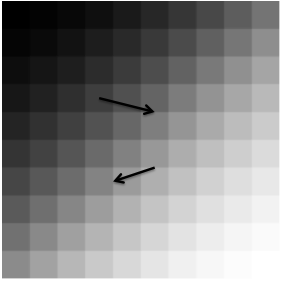
\includegraphics[width=35mm]{use-examples/pointmatching/figures/pairings.png} &
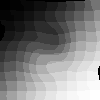
\includegraphics[width=35mm]{use-examples/pointmatching/mosaic-10-10-05.png} \\
&
$(d_p, d_f, \sigma_f) = (10,10,5)$
\end{tabular}
\end{center}
\caption{\label{fig:exe:pointmatching:1} The two pairings superimposed on a mosaic test image, and the resampled image with the deformation computed with $(d_p, d_f, \sigma_f) = (10,10,5)$.}
\end{figure}

The options passed to \pointmatching will be
\begin{code}{1}
-vector-propagation-distance $d_p$
-vector-fading-distance $d_f$
-fluid-sigma $\sigma_f$
\end{code}
where $d_p$, $d_f$, and $\sigma_f$ denotes respectively the propagation distance (of the pairings), the fading distance (of the pairings, after the propagation), and the standard deviation for the regularization (with gaussian interpolation).

Thus, non-linear transformations are computed with different settings for $(d_p, d_f, \sigma_f)$
\begin{code}{1}
\% \pointmatching -flo floating.pts -ref reference.pts -trsf-type vectorfield 
  -template mosaic.mha 
  -vector-propagation-distance $d_p$ 
  -vector-fading-distance $d_f$ 
  -fluid-sigma $\sigma_f$ 
  -res-trsf vectorfield.trsf
\end{code}
and the floating image is resampled thanks to 

\begin{code}{1}
\% \applyTrsf mosaic.mha mosaic-result.mha -trsf vectorfield.trsf -interpolation nearest
\end{code}

\begin{figure}[ht]
\begin{center}
\begin{tabular}{ccc}
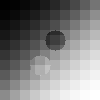
\includegraphics[width=35mm]{use-examples/pointmatching/mosaic-10-00-00.png} &
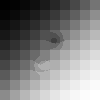
\includegraphics[width=35mm]{use-examples/pointmatching/mosaic-00-10-00.png} &
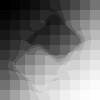
\includegraphics[width=35mm]{use-examples/pointmatching/mosaic-00-00-05.png} \\
$(d_p, d_f, \sigma_f) = (10,0,0)$ &
$(d_p, d_f, \sigma_f) = (0,10,0)$ &
$(d_p, d_f, \sigma_f) = (0,0,5)$ 
\end{tabular}
\end{center}
\caption{\label{fig:exe:pointmatching:2} Vector field deformation computation with only one non-null parameter.}
\end{figure}

On figure \ref{fig:exe:pointmatching:2}, it can be seen that deformations calculated with only one non-null parameter among $(d_p, d_f, \sigma_f)$ lead to non-homotopic deformations. Note that using only $\sigma_f$ should act as pure propagation (except at Vorono\"i diagram borders), but due to numerical reasons, the deformation becomes null when gaussian weights are too small.

\begin{figure}[ht]
\begin{center}
\begin{tabular}{ccc}
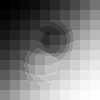
\includegraphics[width=35mm]{use-examples/pointmatching/mosaic-10-10-00.png} &
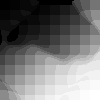
\includegraphics[width=35mm]{use-examples/pointmatching/mosaic-10-00-05.png} &
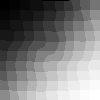
\includegraphics[width=35mm]{use-examples/pointmatching/mosaic-00-10-05.png} \\
$(d_p, d_f, \sigma_f) = (10,10,0)$ &
$(d_p, d_f, \sigma_f) = (10,0,5)$ &
$(d_p, d_f, \sigma_f) = (0,10,5)$ 
\end{tabular}
\end{center}
\caption{\label{fig:exe:pointmatching:3} Vector field deformation computation with only one null parameter.}
\end{figure}

Using two non-null parameters (see figure \ref{fig:exe:pointmatching:3}) allows to get continuous deformations: e.g., $(d_p, d_f, \sigma_f) = (10,0,5)$ and $(d_p, d_f, \sigma_f) = (0,10,5)$. However, deformations may be large at the Vorono\"i diagram borders ($(d_p, d_f, \sigma_f) = (10,0,5)$) or resulting deformations may be quite far away the desired ones ($(d_p, d_f, \sigma_f) = (10,0,5)$). 

Using all the three parameters may yield a deformation close to the expected one (see figure \ref{fig:exe:pointmatching:1}, left). 


